\htmlhr

\newcommand{\theFlowChecker}{the Information Flow Checker\xspace}
\newcommand{\TheFlowChecker}{The Information Flow Checker\xspace}

\chapter{Information Flow Checker\label{flow-checker}}
This chapter describes the Information Flow Checker, a type-checker that 
tracks information flow through your program.
The Information Flow Checker does pluggable type-checking of an information flow type
system.  It is implemented using the Checker Framework.  This chapter is
logically a chapter of the 
Checker Framework Manual (\ifhevea\url{http://types.cs.washington.edu/checker-framework/current/checkers-manual.html}\else\url{http://types.cs.washington.edu/checker-framework/current/checkers-manual.pdf}\fi).
Therefore, in order to understand this chapter, you should first read
chapters 1--2 of the Checker Framework Manual, and you should at least skim
chapters 18--21 (generics through libraries) and 24--25 (FAQ and
troubleshooting). 



To use the Information Flow Checker, a programmer must supply two types of
information:

\begin{itemize}
\item
A flow policy that expresses what information flows the program is allowed
to have. \todo{Why do we need an example here?}  For example, a program might be allowed to send location
information to the network, but not allowed to access contacts nor to send
SMS messages.  The flow policy is primarily derived from the program's user
documentation.  \secref{sec:flow-policy} describes how to write a flow
policy.
\item
\todo{The user doesn't know what a type qualifier is yet, we called them annotations in the overview}
Type qualifiers written on (some of) the variables in the program.  The
type qualifiers indicate where the variable's value came from and where it
might go to.
\end{itemize}

When you run the Information Flow Checker, \todo{ add reference to section that explains how to run Information Flow Checker}it verifies that the annotations in the
program are consistent with what the program's code does, and that the
annotations are consistent with the flow policy.  This gives a guarantee
that the program has no information flow beyond what is expressed in the
flow policy and type annotations.





\section{Flow Policy\label{sec:flow-policy}}

A flow policy is a list of all the information flows that are permitted to occur
in an application.
A flow policy file expresses a flow policy, as a list of $\flow{\|flowsource|^*}{\|flowsink|^*}$ pairs.
Just as the Android manifest lists all the permissions that an app uses,
the flow policy file lists the flows among permissions and other sensitive 
locations. 

\subsection{Semantics of a Flow Policy}
\label{sec:undsiredflows}
The Information Flow Checker guarantees that there is no information
flow except for what is explicitly permitted by the policy file. If a user writes a type that is
not permitted by the policy file, then the Information Flow Checker issues a warning
even if all types in program otherwise typecheck.

For example, this variable declaration

\begin{alltt}
@Source(CAMERA) @Sink(INTERNET) Video video = ...
\end{alltt}

\noindent
is illegal unless the the policy file contains:

\begin{alltt}
CAMERA -> INTERNET
\end{alltt}

Here is another example.
The flow policy file contains:
\begin{alltt}
  ACCOUNTS      -> EXTERNAL_STORAGE, FILESYSTEM
  ACCELEROMETER -> EXTERNAL_STORAGE, FILESYSTEM, INTERNET
\end{alltt}

The following variable declarations are permitted:
\begin{alltt}
  @Source(ACCOUNTS) @Sink(EXTERNAL_STORAGE) Account acc = ...
  @Source({ACCELEROMETER, ACCOUNTS})
  @Sink({EXTERNAL_STORAGE, FILE_SYSTEM}) int accel = ...
\end{alltt}

The following definitions would generate ``forbidden flow'' errors:
\begin{Verbatim}
  @Source(ACCOUNTS) @Sink(@INTERNET) Account acc = ...
  @Source({ACCELEROMETER, ACCOUNTS})
  @Sink({EXTERNAL_STORAGE, FILESYSTEM, INTERNET})
\end{Verbatim}

\myparagraph{Transitivity and the flow policy file}
\label{sec:flow-policy-transitivity}
The flow policy file indicates specific permitted information flows.  It
may be possible to combine these flows.
For example, a policy that permits
\flow{CAMERA}{FILESYSTEM} and \flow{FILESYSTEM}{INTERNET}
will implicitly allow the flow \flow{CAMERA}{INTERNET},
because the application may record from the camera into a file
and then send the contents of the file over the network.
\TheFlowChecker forbids such implied flows:  the developer is required to write
the transitive flow in the flow policy file, which requires the developer
to justify its purpose or convince the app store that the flow is not used.
%Finer-grained permissions, as discussed in
%\secref{sec:future}, would reduce the impact of implied flows.
\todo{Explain/show warning}


\subsection{Syntax of a Flow Policy File}

Each line of a policy file specifies a permitted flow from a source to one
or more sinks.  For example,
\code{MICROPHONE -> INTERNET} implies that
MICROPHONE data is always allowed to flow to INTERNET.
The source or sink must be a member of the enum
\<sparta.checkers.quals.FlowPermission>.  
ANY is allowed just as it is in @Source and @Sink, but empty, \ttcbs, is not allowed.

Multiple sinks can appear on the same line if they are separated by commas. 
For example,
this policy file:
\begin{alltt}
   MICROPHONE -> INTERNET, LOG, DISPLAY
\end{alltt}
is equivalent to this policy file:
\begin{alltt}
   MICROPHONE -> INTERNET
   MICROPHONE -> LOG
   MICROPHONE -> DISPLAY, INTERNET
\end{alltt}

The policy file may contain blank lines and comments that begin with 
a number sign (\<\#>) character.



\subsection{Using a flow-policy file}
To use a flow-policy file when invoking the Information Flow Checker from the
command line, pass it the option:
\begin{alltt}
-AflowPolicy=\emph{mypolicyfile}
\end{alltt}

Or if you are using the \<check-flow> ant target, you can pass the option to ant:
\begin{alltt}
ant -DflowPolicy=\emph{mypolicyfile} check-flow
\end{alltt}
If the flow policy is named \<flow-policy> and is located the top level app directory, the ant 
target will use it automatically.






\section{Source and Sink annotations\label{sec:flow-type-system}}


The type qualifier \<@Source> on a variable's
type indicates what sensitive sources might affect the variable's value.
The type qualifier \<@Sink> indicates where (information computed from) the
value might be output.
These qualifiers can be used on any occurrence
of a type, including in type parameters, object instantiation, and cast types.


As an example, consider the declaration

\begin{Verbatim}
    @Source(LOCATION) @Sink(INTERNET) double loc;
\end{Verbatim}

\noindent
The type of variable \<loc> is \<@Source(LOCATION) @Sink(INTERNET)
double>.
The \<@Source(LOCATION)> qualifier indicates that the
value of \<loc> might have been derived from
location information.
Similarly, the qualifier \<@Sink(INTERNET)> indicates that
\<loc> might be output to the network.  It is also
possible that the data has already been output.
A programmer typically writes either \<@Source> or \<@Sink>, but not both, as explained
in  \secref{sec:system:defaults}. 

The arguments to \<@Source> and \<@Sink> are one or more permissions
drawn from our enriched permission system (\secref{sec:permissions}).
The rarely-used special constant \<ANY> denotes the set of all sources or the set of all
sinks.
%Most of them correspond to Android permissions (see 
%\url{http://developer.android.com/reference/android/Manifest.permission.html}),
%and others are new ``permissions'' that provide finer-grained control over
%the behavior of an application.

\subsection{FineSource and FineSink Annotations\label{sec:fine-source-and-sink}}
\<@FineSource> and \<@FineSink> annotations follow the same conventions as 
regular \<@Source> and \<@Sink> annotations. However, they are embedded within
the respective \<@Source> and \<@Sink> annotations that are being parameterized.
That is, \<@Source> and \<@Sink> annotations have optional attributes for
finesources and finesinks, respectively. Each FineSource and FineSink annotation
takes a value attribute consisting of the coarse FlowPermission to be parameterized.
Each finer grained annotation also has a params attritibute, which is a
string list of parameters associated with the finer-grained permission.

As an example, we parameterize the example declaration above
\begin{Verbatim}
    @Source(LOCATION) 
    @Sink(finesinks={@FineSink(value=INTERNET, params={"mydomain.org"})}) double loc;
\end{Verbatim}

\subsection{Subtyping\label{sec:subtyping}}

\begin{figure}
\centerline{\includegraphics[width=.49\textwidth]{figures/flowsources}%
  \hfill%
  \includegraphics[width=.49\textwidth]{figures/flowsinks}}
\caption{Partial qualifier hierarchy for flow source and flow sink type
  qualifiers, expressed as Java annotations \<@Source> and \<@Sink>.}
\label{fig:flow-hierarchy}
\end{figure}


A type qualifier hierarchy indicates
which assignments, method calls, and overridings are legal, according to
standard object-oriented typing rules.
\figref{fig:flow-hierarchy} shows parts of the \<@Source> and
\<@Sink> qualifier hierarchies.


\<@Source($B$)> is a subtype of \<@Source($A$)> iff \<$B$> is a subset of \<$A$>.
For example, \<@Source(INTERNET)> is a subtype of \<@Source(\{INTERNET, LOCATION\})>.
This rule reflects the fact that the \<@Source> annotation
places an upper bound on the set of sensitive sources that were actually
used to compute the value.
If the type of \<x> contains \<@Source(\{INTERNET, LOCATION\})>, then the value
in \<x> might have been derived from both \<INTERNET> and \<LOCATION> data, or
only from \<INTERNET>, or only from \<LOCATION>, or from no
sensitive source at all.
% XXX

The opposite rule applies for sinks:
\<@Sink($B$)> is a subtype of \<@Sink($A$)> iff \<$A$> is a subset of \<$B$>.
The type \<@Sink(\{INTERNET, LOCATION\})> indicates that
the value is permitted to flow to both \<INTERNET> and \<FILESYSTEM>.  This
is a subtype of \<@Sink(INTERNET)>, as the latter type provides fewer routes through which the information may be
leaked.

\subsubsection{Subtyping for parameterized sources and sinks\label{sec:param-subtyping}}

\begin{figure}
\centerline{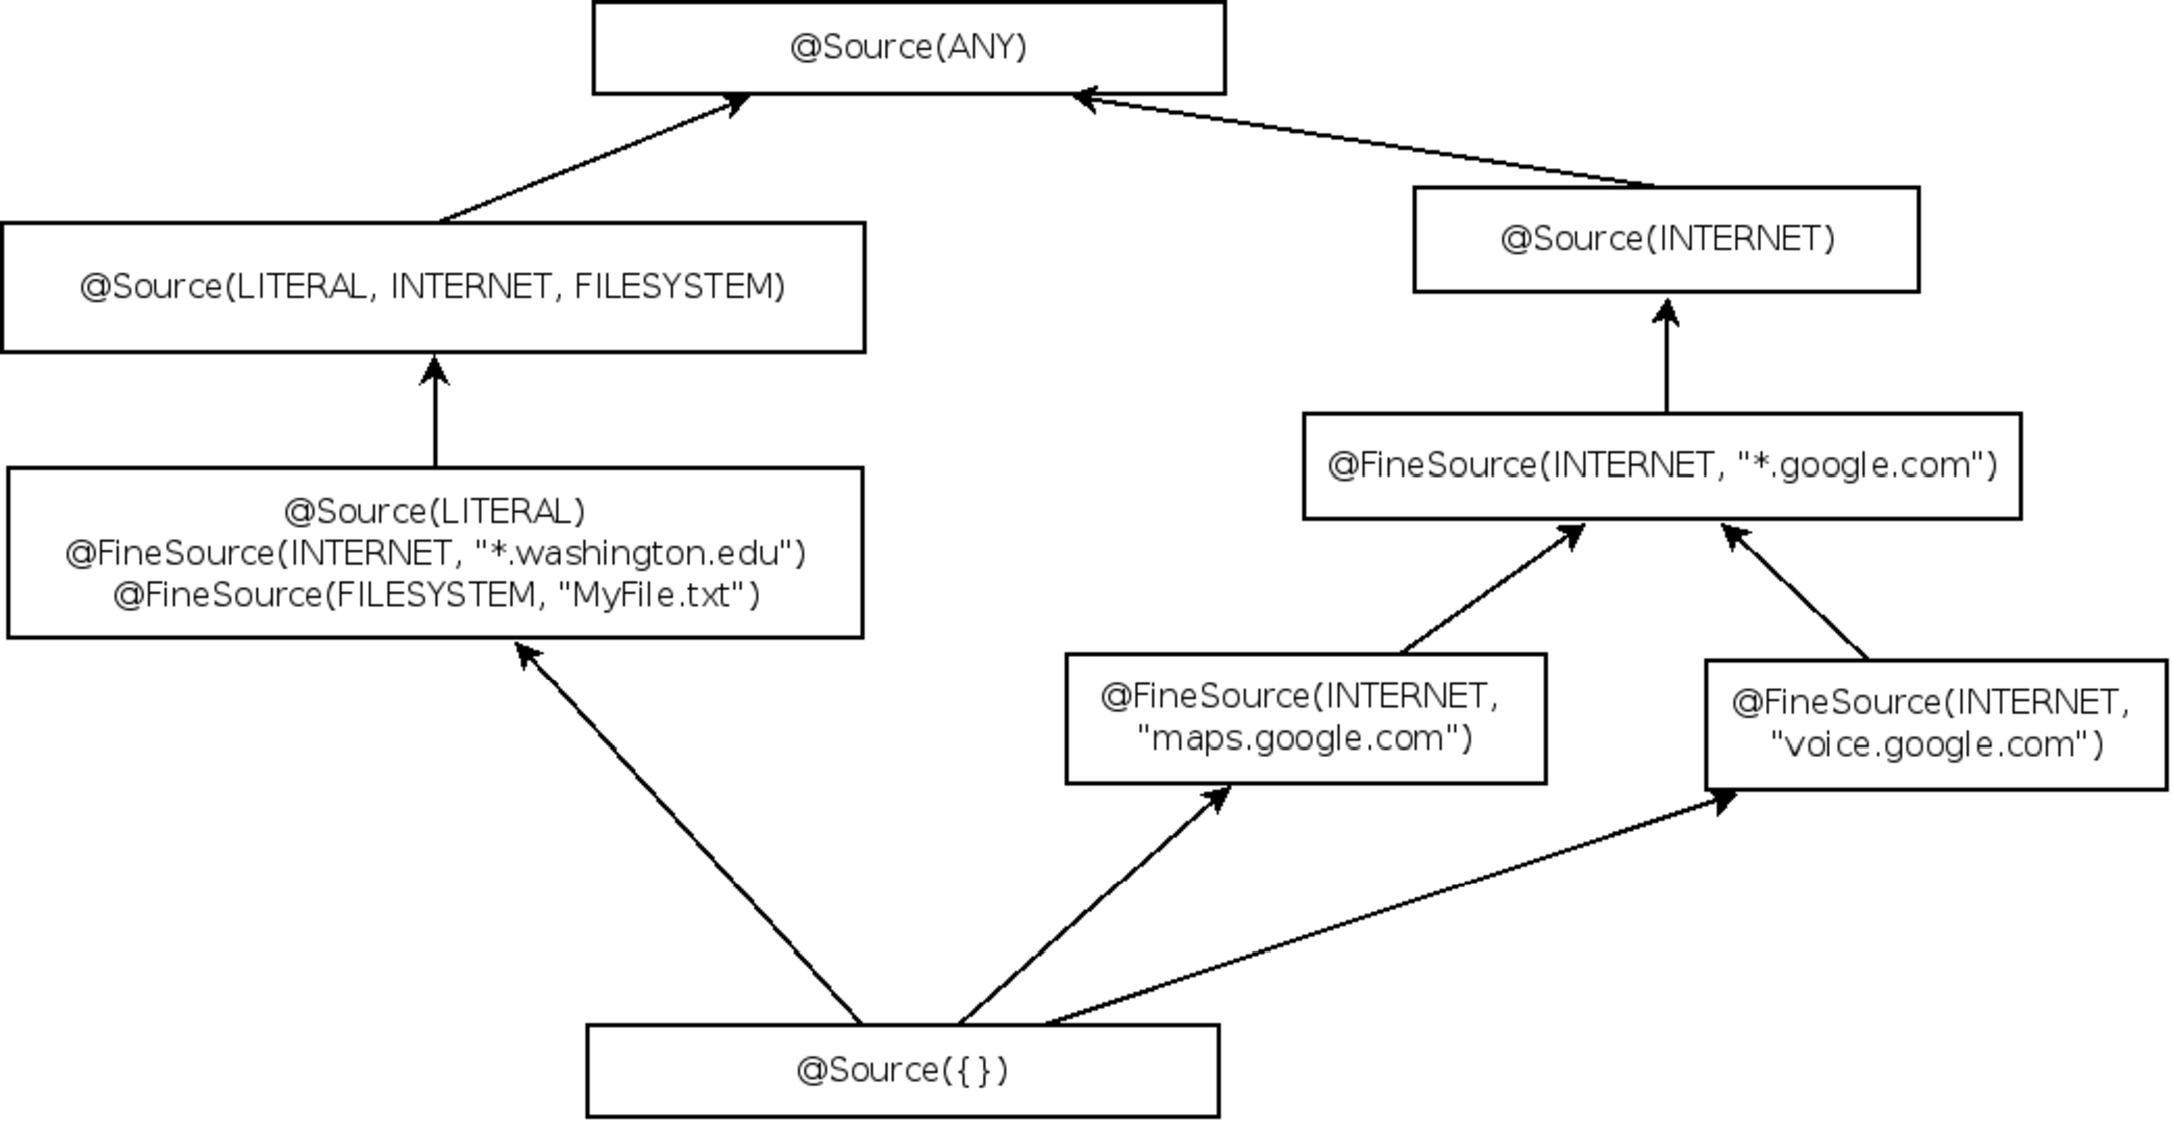
\includegraphics[width=1.0\textwidth]{figures/flowsources_parameterized}}
\caption{Partial qualifier hierarchy for parameterized flow source type
  qualifiers, expressed as Java annotations \<@FineSource>.}
\label{fig:flow-hierarchy-parameterized-source}
\end{figure}

\begin{figure}
\centerline{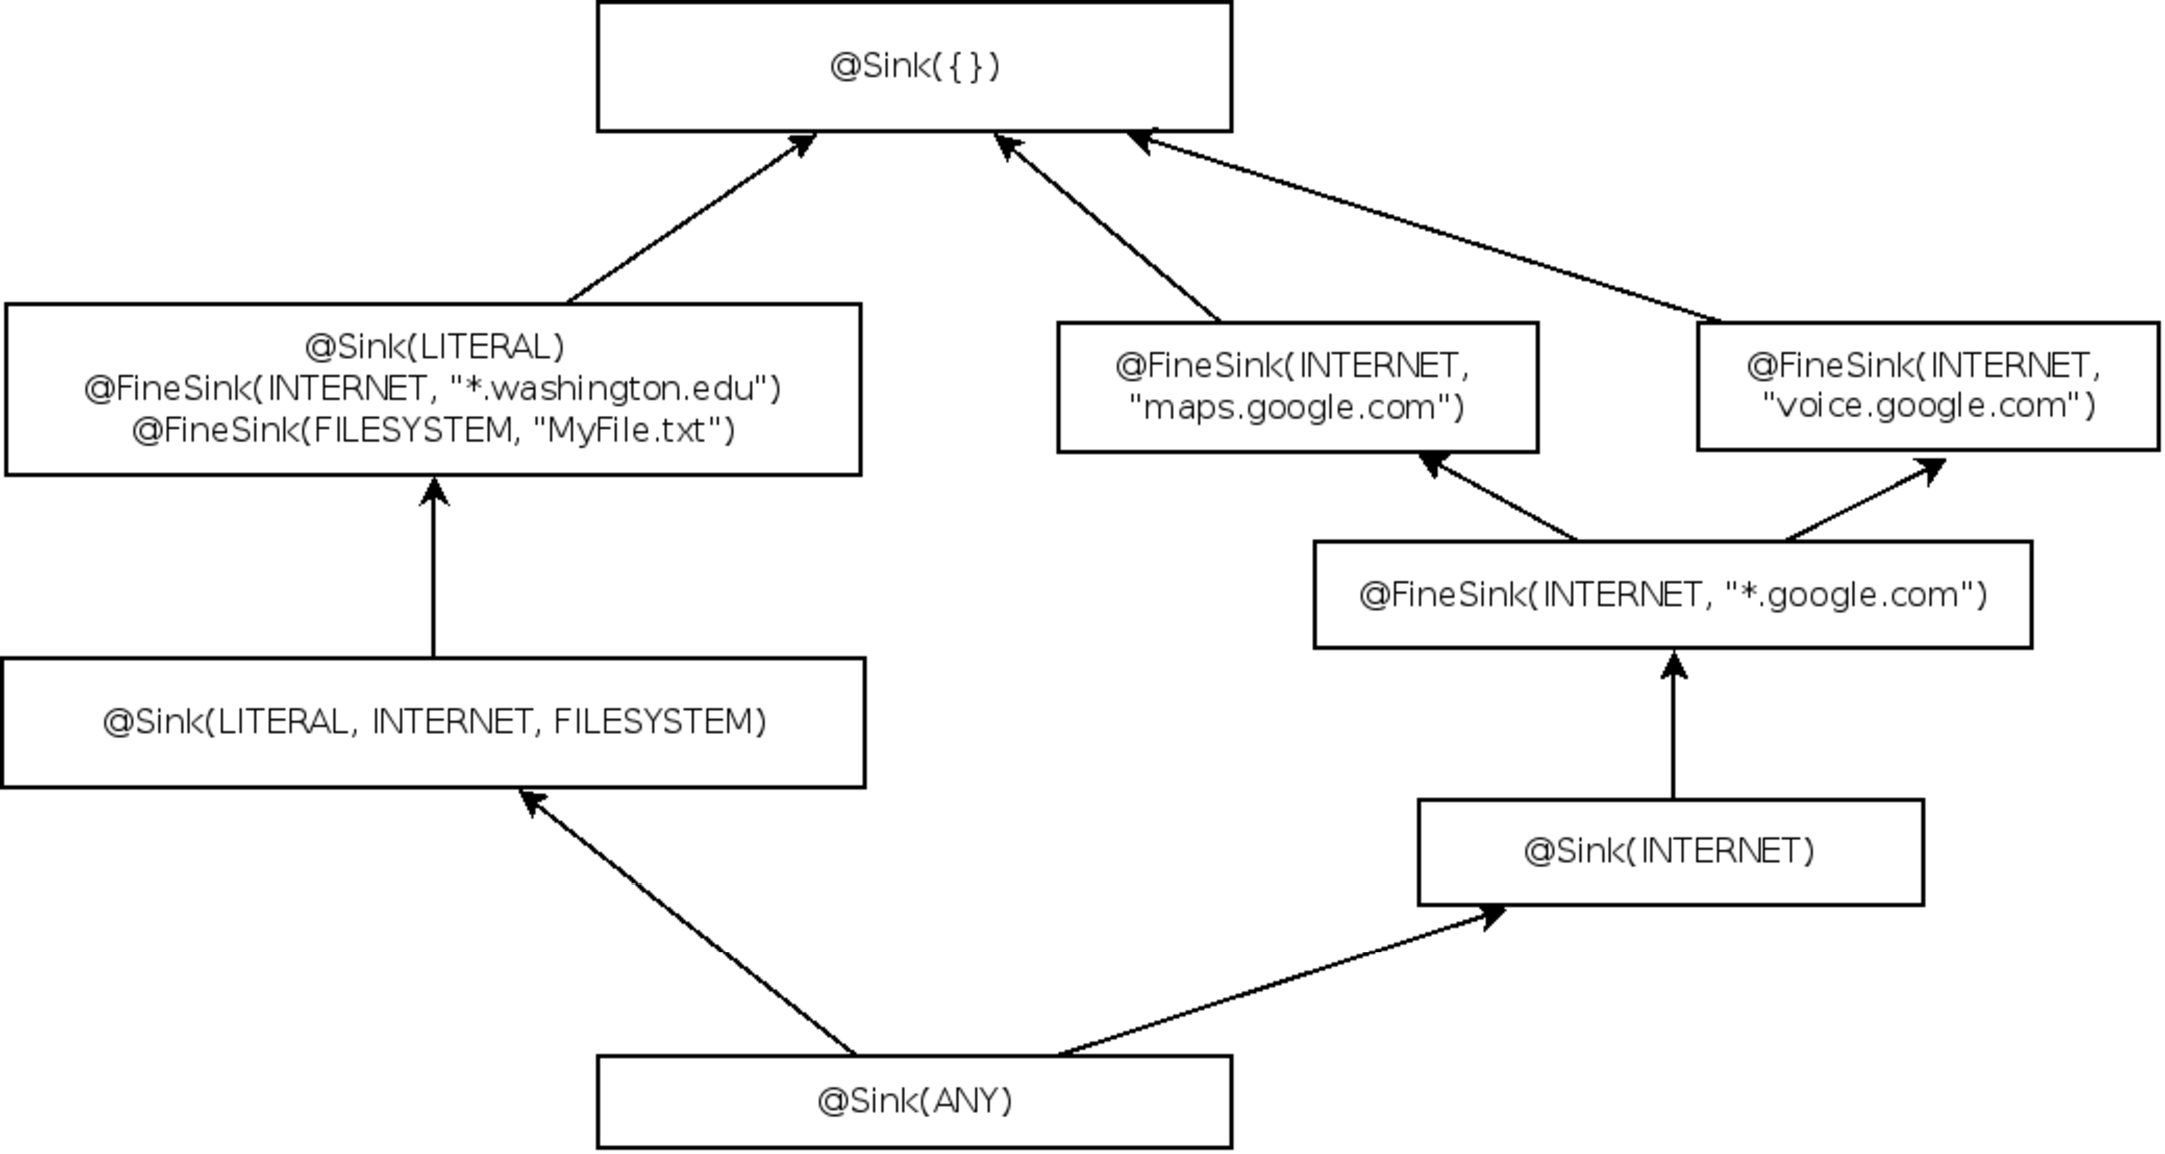
\includegraphics[width=1.0\textwidth]{figures/flowsinks_parameterized}}
\caption{Partial qualifier hierarchy for parameterized flow sink type
  qualifiers, expressed as Java annotations \<@FineSink>.}
\label{fig:flow-hierarchy-parameterized-sink}
\end{figure}

Subtyping rules for parameterized permissions extend the subtyping rules for
non-parameterized permissions. All non-parameterized permissions will default
to having ("*") for its parameter. The asterisk(*) will be treated as a wildcard
for purposes of subtyping, so non-parameterized permissions will subsume all
its parameterized counterparts. 

\noindent
@FineSource(X,{"B1", "B2", ..."BN"}) is a subtype of @Source(Y, {"A1", "A2", ..."AN"}), 
if:
\begin{Verbatim}
  1. X and Y are the same permission
  2. for each string B parameter in {"B1", "B2", ..."BN"}
        for each string A in {"A1", "A2", ..."AN"}
          if(A is a regex and B is a string)
             B must match A
          if(A is a string and B is a string)
             B must be the same A
          if(A is a regex and B is a regex)
             B must be contained by A
          if(A is a string and B is a regex)
              //B is not a subtype of A
\end{Verbatim}

For example, Source(FILESYSTEM("/tmp/*")) is a supertype of FILESYSTEM("/tmp/file.txt")\newline

\noindent
@FineSink(X,{"B1", "B2", ..."BN"}) is a subtype of @FineSink(Y, {"A1", "A2", ..."AN"}), 
if:
\begin{Verbatim}
  1. A and B are the same permission
  2.  for each string A in {"A1", "A2", ..."AN"}
        for each string B in {"B1", "B2", ..."BN"}
          if(A is a string and B is a regex)
             A must match B
          if(A is a string and B is a string)
             A must be the same B
          if(A is a regex and B is a regex)
             A must be contained by B
          if(A is a regex and B is a string)
            //B is not a subtype of A
\end{Verbatim}
For example, a flow of 'SMS -> INTERNET("*.google.com")' is a subtype of 
'SMS -> INTERNET("maps.google.com")' because the supertype's value is a match to 
the subtype's regular expression.

\section{Comparison to Android permissions}
\label{sec:permissions}


\TheFlowChecker is finer-grained than standard Android manifest permissions
in two ways.  First, Android permits any flow
between any pair of permissions in the manifest --- that is, any resource
mentioned in the manifest may be used in an arbitrary way.
  In contrast, the Information Flow Checker enforces the information flows in the flow policy.
Second,
\theFlowChecker uses finer-grained permissions than Android does, in
particular by adding additional permissions.
Such finer-grained analysis is necessary in order to detect Trojans that would 
look innocuous, given Android's coarser model.
For example, \theFlowChecker requires 
a permission to retrieve data from the accelerometer, which can indicate the user's
physical activity, and to retrieve the time of day, which can be used
as a trigger for malicious behavior.

Our system does not add much complexity:  it only adds 28 permissions to
Android's standard 130, or 22\% more permissions.  \tabref{tab:perms} lists
the additional permissions.

%Some researchers feel that the Android permission model is already too complicated for
%users to understand~\cite{felt:2011:permissions}.  But our perspective is that of an auditor who
%is trained to analyze an application.  The flow policy is examined once
%per application by a skilled engineer, not on every download by a user, so
%the total human burden is less.  The more detailed flow
%policy file may even be more comprehensible than simple Android permissions,
%because the flow policy makes clear how each resource is used, not just
%that it is used.

\begin{table}
\caption{Additional permissions used by \theFlowChecker, beyond the built-in 130 Android permissions.}
%\setlength{\tabcolsep}{.5\tabcolsep}
\begin{tabular}{lll}
\hline
\textbf{Sources}     &\textbf{Sinks}     &\textbf{Both source and sink}\\
\hline
ACCELEROMETER     &DISPLAY     &CAMERA\_SETTINGS\\
BUNDLE     &SPEAKER     &CONTENT\_PROVIDER\\
MEDIA     &WRITE\_CLIPBOARD     &DATABASE\\
PHONE\_NUMBER     &WRITE\_EMAIL     &FILESYSTEM\\
RANDOM     &WRITE\_LOGS     &INTENT\\
READ\_CLIPBOARD     &&PARCEL\\
READ\_EMAIL     &&PROCESS\_BUILDER\\
READ\_TIME     &&SECURE\_HASH\\
REFLECTION     &&SHARED\_PREFERENCES\\
SENSOR     &&SQLITE\_DATABASE\\
USER\_INPUT     &&SYSTEM\_PROPERTIES\\
\end{tabular}
\label{tab:perms}
\end{table}

%  LocalWords:  FILESYSTEM SQLITE


We now discuss two permissions, \perm{LITERAL} and \perm{CONDITIONAL}, and empty  whose meaning may not be obvious.

\subsubsection{Literals}
The \perm{LITERAL} source is used for programmer-written manifest
constants, such as \<"Hello world!">.
This enables \theFlowChecker to distinguish information derived
from the program source code from other inputs.
Manifest literals are used benignly for many 
purposes, such as configuring default settings.
The flow policy shows the ways they are used in the program, and they can
be directly examined by the analyst.


\subsubsection{Conditionals \label{sec:conditionals}}
\TheFlowChecker treats conditional statements as a flow sink
to enable detection of indirect flows that leak private information.
For example, without any treatment of conditionals, the following code would
be permitted under a flow policy containing \flow{LITERAL}{INTERNET} and \flow{USER\_INPUT}{FILESYSTEM}:

\begin{Verbatim}
    @Source(USER_INPUT) @Sink(FILESYSTEM)
    long creditCard = getCCNumber();
    final long MAX_CC_NUM = 9999999999999999;
    for (long i = 0 ; i < MAX_CC_NUM ; i++) {
        if (i == creditCard)
            sendToInternet(i);
    }
\end{Verbatim}

To prevent malicious developers from bypassing the type system in this manner,
\theFlowChecker requires the type of a
conditional expression to include the sink \perm{CONDITIONAL}.
By default, literals are allowed to flow
to a conditional; that is, \flow{LITERAL}{CONDITIONAL} is added to the flow policy by default.

Data containing sensitive information is often passed through conditional statements for benign reasons.  
For example, an app might verify that a credit card number entered is valid by checking the number of digits.

\begin{Verbatim}
    @Source(USER_INPUT) @Sink(FILESYSTEM)
    long creditCard = getCCNumber();
    final long MAX_CC_NUM = 9999999999999999;

    if (MAX_CC_NUM < creditCard)
        reportTooManyDigits();
\end{Verbatim}

In this case, the credit card number is not indirectly leaked, but \theFlowChecker  
cannot determine this and will report a false positive.
The auditor must examine the code nearby
to ensure that the conditional is not being used to indirectly leak information.


\subsubsection{Empty sink or source\label{sec:emptyflow}}

Programmers may not use @Source(\ttcbs) or @Sink(\ttcbs).
Every value should either flow from a literal or from some sensitive
source.  Likewise, every value must flow to a sensitive sink or to a
conditional expression.  Any variable that does not have
 a flow sink does not actually affect the output of the program and
should therefore be removed.
  
Note that this does not mean you must specify both a flow source
annotation and a flow sink annotation as explained in
\secref{sec:system:defaults}. 

  \section{Inference and defaults}
 \label{sec:system:defaults}
 
 A complete type consists of a \<@Source> qualifier, a \<@Sink> qualifier,
 and a Java type.  To reduce programmer effort and code clutter, most of the
 qualifiers are inferred or defaulted.  
 
 A programmer need not write qualifiers within method bodies,
 because such types are inferred by \theFlowChecker (see \secref{sec:type-inference}).
 Even for method signatures and
 fields, a programmer generally writes either \<@Source> or
 \<@Sink>, but not both; see \secref{sec:infer-from-flow-policy} and 
\secref{sec:unannotated-types}.

\subsection{Local variable type inference}
\label{sec:type-inference}

A programmer does not write information flow types within method bodies.  Rather, local
variable types are inferred.

We limit type inference to local variables to ensure that
each method can be type-checked in isolation,
with a guarantee that the entire program is type-safe if each method has
been type-checked.  It would be possible to perform a whole-program type
inference, but such an approach would not be modular, would be
heavier-weight, would not deal well with cooperating or communicating
applications, and would provide fewer documentation benefits.  


\subsection{Determining sources from sinks and vice versa}
\label{sec:infer-from-flow-policy}

If a type contains only a flow source or only a flow sink, the other qualifier is
filled in with the most general one that is consistent
with the policy file.
%
If the programmer writes 
\<@Source($\alpha$)>, \theFlowChecker defaults this to
\<@Source($\alpha$)> \<@Sink($\omega$)> where $\omega$ is the
set of flow sinks that all sources in $\alpha$ can flow to.
%
Similarly,
\<@Sink($\omega$)> is defaulted to
\<@Source($\alpha$)> \<@Sink($\omega$)> where $\alpha$ is the
set of flow sources allowed to flow to all sinks in $\omega$.
%
Defaults are not applied if the programmer writes both a source and a
sink qualifier.

For example, suppose the flow policy contains the following:

\begin{Verbatim}
    A -> X,Y
    B -> Y
    C -> Y
\end{Verbatim}
  
\noindent 
Then these pairs are equivalent:
\begin{eqnarray*}
  \mbox{\<@Source({B,C})>} & = & \mbox{\<@Source({B,C}) @Sink(Y)>} \\
  \mbox{\<@Sink(Y)>}       & = & \mbox{\<@Source({A,B,C}) @Sink(Y)>}
\end{eqnarray*}

This mechanism is useful because oftentimes a programmer thinks about a
computation in terms of only its sources or only its sinks.
The programmer should not have to consider the rest of the program
that provides context indicating the other end of the flow.

\newcommand{\FCnumstubmethods}{10,553\xspace}
\newcommand{\FCnumstubmethodsrounded}{10,000\xspace}
% Number of stub file methods with explicit @Source and/or @Sink annotations
% on some argument or the return type or receiver.  (The remaining methods use
% some variant of @PolyFlow.)
\newcommand{\FCnumstubmethodswitheither}{915\xspace}
% Number of stub file methods with both @Source and @Sink annotations
\newcommand{\FCnumstubmethodswithboth}{76\xspace}
% numstubmethodswitheither / numstubmethodswithboth, as a percentage
\newcommand{\FCpercentstubmethodswithboth}{8\%\xspace}
\newcommand{\FCpercentstubmethodswithone}{92\%\xspace}

This defaulting mechanism is essential for annotating
libraries.  \TheFlowChecker ships with manual annotations for more than
\FCnumstubmethodsrounded methods of the Android standard library.
%% Mike tweaked the wording.  I hope it's still accurate.
% Of the
% % \FCnumstubmethodswitheither
% methods with explicit \<@Source> or \<@Sink> annotations,
\FCpercentstubmethodswithone of methods use only a
\<@Source> or \<@Sink> annotation but not both.
% \todo{These numbers are weird:  if only \FCnumstubmethodswitheither have \<@Source> or \<@Sink>, what about the other 9,000+ methods?  Were they manually-verified to not required any annotation?  That should be clarified here.}
An example is the \<File> constructor:
a newly-created readable file should be annotated with
\<@Source(FILESYSTEM)>, but there is no possible \<@Sink> annotation
that would be correct for all programs.
Instead, the \<@Sink> annotation is omitted, and
our defaulting mechanism provides the correct value
based on the application's flow policy.



\subsection{Defaults for unannotated types}
\label{sec:unannotated-types}


\begin{table}
  \caption{Default information-flow qualifiers for unannotated types}
  \begin{tabular}{l l}
  \hline
    \bf{Location} & \bf{Default Flow Type}\\
  \hline
     \<@Source($\alpha$)>&\<@Source($\alpha$)>
       \<@Sink($\omega$)>,  $\omega$ is the set of  sinks allowed to flow from all sources in $\alpha$ \\
     \<@Sink($\omega$)>&\<@Source($\alpha$)>
       \<@Sink($\omega$)>, $\alpha$ is the set of  sources allowed to flow to all sinks in $\omega$ \\
    Method parameters &  \<@Sink(CONDITIONAL)> \\
    Method receivers &  \<@Sink(CONDITIONAL)> \\
    Return types &  \<@Source(LITERAL)> \\
    Fields &  \<@Source(LITERAL)> \\
    \<null> &  \<@Source(\{\}) @Sink(ANY)>\\
    Other literals & \<@Source(LITERAL) >\\
    Type arguments & \<@Source(LITERAL) >\\
    Local variables &   \<@Source(ANY) @Sink(\{\})> \\
    Upper bounds &   \<@Source(ANY) @Sink(\{\})> \\
    Resource variables  &   \<@Source(ANY) @Sink(\{\})> \\
  
  \end{tabular}

  \label{tab:defaults}
\end{table}

Table \ref{tab:defaults} shows defaults for completely unannotated types.
\TheFlowChecker allows a developer to choose a different default for a
particular method, class, or package.
When the default is only a source or only a sink, the other qualifier is
inferred from the policy file as explained in
\secref{sec:infer-from-flow-policy}.

Most unannotated types (including field types, return
types, generic type arguments, and non-\<null>
literals) are given the qualifier \<@Source(LITERAL)>.  
This is so that simple computation involving manifest literals, but not
depending on Android permissions, does not require 
annotations. 

As is standard, the \<null> literal is given the bottom type qualifier, which allows it to be assigned to any variable.
For \theFlowChecker, the bottom type qualifier is \srcnone\  \<@Sink(ANY)>.



\section{Warning suppression\label{sec:waringsuppression}}
 
Sometimes it might be necessary to suppress warnings or errors produced by
the Information Flow Checker.  This can be done by using the
\<@SuppressWarnings("flow")> annotation on a variable, method, or (rarely)
class declaration.  Because this annotation can be used to subvert the Flow
Checker, its use is considered suspicious.  Anytime a warning or error is
suppressed, you should write a brief comment justifying the suppression.
\<@SuppressWarnings("flow")> should only be used if there is no way to
annotate the code so that an error or warning does not occur.  

\section{Annotating library API methods in stub files\label{sec:apispecs}}

Annotations for API methods are found in the stub files in sparta-code/src/sparta/checkers/flowstubfiles.
For details, see Section~\ref{flow-task-annotate-apis} of this manual, and also 
chapter
``\ahref{\url{http://types.cs.washington.edu/checker-framework/current/checkers-manual.html#annotating-libraries}}{Annotating
  Libraries}'' in the Checker Framework Manual.  
 The methods that appear in stub files are defaulted the same way as methods 
written in apps, including flow policy inference.  
(See the defaulting section, \secref{sec:system:defaults}.) 

  The Information Flow Checker  outputs all of the methods missing from the stub files in
  a file called \<missingAPI.astub> in the current working directory. It also 
  contains a comment the number of times an API method is used by the app.

Any method not written in the stub files or found in source code is not defaulted normally. 
 Instead, its return, receiver, and parameter types are annotated with \<@Sources(NOT\_REVIEWED)> 
 \<@Sinks(NOT\_REVIEWED)>. 
 This way, if such an API method is used, a type error
  will occur and alert the user to review and annotate the method. It is possible, but dangerous, to ignore these kind of warnings as explained in \secref{sec:run-type-checker}.


\section{Polymorphism \label{sec:polyflowsources}}


Information flow type qualifiers interact seamlessly with parametric polymorphism (Java
generics).  For example, a programmer can declare

\begin{Verbatim}
    List<@Source(CONTACTS) @Sink(SMS) String> myList;
\end{Verbatim}
\noindent
Here, the elements of \<myList> are strings
that are obtained from \<CONTACTS> and that may flow to \<SMS>.

\TheFlowChecker also supports qualifier polymorphism, in
which the type qualifiers can change independently of the underlying type.
This allows a programmer to write a generic method that can operate on values of
any information flow type.
For example, if a method is declared as
\<@PolySource int f(@PolySource int x)>, then it can be called on an \<int>
with any flow sources, and the result has exactly the same sources as the
input.  This can be viewed as a declaration and two uses of a type
qualifier variable.  The implicit type qualifier variables are
automatically instantiated by \theFlowChecker at the point of use.

For brevity,
the additional
annotation \<@PolyFlow> can be written on a class or method declaration to indicate that
all contained parameters and return types should be annotated as \<@PolySource
@PolySink>.  \<@PolyFlow> does not override explicitly-written annotations as explained
in \secref{sec:polyflow}.


Parametric polymorphism, qualifier polymorphism, and regular Java types can
be used together.  The type system combines the
qualifier variables and the Java types into a complete qualified type.

See section ``\ahref{http://types.cs.washington.edu/checker-framework/current/checkers-manual.html#qualifier-polymorphism}{Qualifier polymorphism}'' in the Checker Framework Manual.  

% These range over their respective type hierarchy and can be used to
% express type dependencies, for example, that the receiver and
% parameter types have to correspond.
% The invocation of a method is used to resolve polymorphic qualifiers
% to something concrete.

\todo{these have known soundness issues and with Stuart we're working on fixing them.}


\section{Declaration annotations to specify defaulting\label{sec:addtionalanno}}

The Information Flow Checker has additional declaration annotations that are shorthand for common 
annotation patterns on method signatures.   They override the usual defaulting of method declarations.

\subsection{@PolyFlow\label{sec:polyflow}}

Annotation \<@PolyFlow> expresses that each contained method should be annotated as \<@PolySource> 
\<@PolySink> for both the return types and all parameters. It should be used to express a relationship 
between the return type and the parameter types, but not the receiver type.


\subsection{@PolyFlowReceiver\label{sec:polyflowreceiver}}

Annotation \<@PolyFlowReceiver> expresses that each contained method should be annotated as \<@PolySource> \<@PolySink> for the return type, all parameter types, and the receiver type.

\subsection{Declaration annotations in stub files\label{sec:declannosstubfiles}}
If \<@PolyFlow> or \<@PolyFlowReceiver> is written on a class or package, then the annotation applies
 to all contained methods or classes unless those classes or methods are annotated with another 
 declaration annotation.   

This change of defaulting happens to library methods that are not written in stub files.  For example, the class
 Integer as been annotated with  \<@PolyFlowReceiver>, but the toString method is not listed in the stub file.  
 This method is inferred to be annotated with  \<@PolyFlowReceiver> and therefore its use will not result in a 
 type error  involving the \<NOT\_REVIEWED> FlowPermission. 
 






\section{Stricter tests\label{sec:stricter}}

By default, the Information Flow Checker is unsound.  After getting the basic checks to pass, the
 stricter checks should be enabled, by running \<ant -Dsound=true check-flow>.
This two-phase approach was chosen to reduce
the annotation effortand to give two separate phases of
the annotation effort.
 The sound checking enforces invariant 
array subtyping and type safety in downcasts.


When strict checks are turned on,
a cast \<(Object []) x>, were \<x> is of type \<Object>, will result
in a compiler warning:

\begin{alltt}
[jsr308.javac] ... warning: "@Sink @Source({ANY}) Object"
       may not be casted to the type "@Sink @Source Object"
\end{alltt}

The reason is that there is not way for the type-checker to verify
 the component type of the array. There is no static knowledge about the actual
runtime values in the array and important flow could be hidden.
The analyst should argue why the downcast is safe.

Note that the main qualifier of a cast is automatically flow-refined
by the cast expression.


\medskip

Stricter checking also enforces invariant array subtyping, which is
needed for sound array behavior in the absence of runtime checks.
Flow inference automatically refines the type of array creation
expressions depending on the left-hand side.

\medskip

Enabling stricter checking will also enable the \<-Alint=strict-conditional> option to limit 
allowed sinks to conditionals.

\section{Guidance on writing annotations}
\chapref{tutorial} is a tutorial on how to annotate an existing application. 
See \chapref{app-annotation} for tips about
writing information-flow annotations. 

%\section{Miscellaneous\label{sec:miscellaneous}}

%Some methods that are intended to be overridden by subclasses, such as 
%\<Object>'s \<equals()> and \<toString()>, are given the most general
%possible return type, \<@Source(ANY) @Sink({})>.
%\todo{ Is this rationale correct??}
%This permits overriding methods to give them a more specific return type, which
%might depend on fields of the overriding class as well as on the types of
%the arguments.  In fact, an overriding method must give a more specific
%return type, since \<@Sink> prevents the value from being used.

%Most binary operations, such as string concatenation and integer addition,
%produce a result whose type is the least upper bound of the two operand types.


%% Adding on to that, if you try to compute a @FlowPermission{something} int
%%  with a int literal (0 or 100, etc) it will resolve to another
%%  @FlowPermission{something} int. If you try the same with a
%%  @FlowPermission{something} int with an int literal, it will result in
%%  @FlowPermission{} int because it's not safe to add a flowsink to the int
%%  literal. To bypass this, you must declare a local variable with
%%  "@SuppressWarnings("flow") @FlowPermission{something} int tempZero = 0;"
%%  and then use the local variable in the calculation.
%%  Again document why the warning can be suppressed.


%%% Local Variables: 
%%% mode: latex
%%% TeX-master: "manual"
%%% TeX-command-default: "PDF"
%%% End: 

%  LocalWords:  Sink someData Source enum 5cm flowsources 'c'
%  LocalWords:  flowsinks realString asdf PolySource PolySink
%  LocalWords:  sparta NoFlow ConservativeFlow astub TODO jsr308
%  LocalWords:  FlowPermission
